\documentclass[aspectratio=43]{beamer}

% Text packages to stop warnings
\usepackage{lmodern}
\usepackage{textcomp}
\usepackage{ulem}
\usepackage[utf8]{inputenc}
\usepackage[T1]{fontenc}

\usepackage{listings}
\usepackage{tikz}
\usetikzlibrary{arrows,decorations.pathreplacing,positioning}

% Themes
\usetheme{Boadilla}
\setbeamertemplate{footline}[page number]{}
\setbeamertemplate{navigation symbols}{}

% Suppress the navigation bar
\beamertemplatenavigationsymbolsempty

\newenvironment{changemargin}[1]{% 
  \begin{list}{}{% 
    \setlength{\topsep}{0pt}% 
    \setlength{\leftmargin}{#1}% 
    \setlength{\rightmargin}{1em}
    \setlength{\listparindent}{\parindent}% 
    \setlength{\itemindent}{\parindent}% 
    \setlength{\parsep}{\parskip}% 
  }% 
  \item[]}{\end{list}} 

\lstset{basicstyle=\scriptsize, frame=single}

\lstdefinelanguage{JavaScript}{
  keywords={typeof, new, true, false, catch, function, return, null, catch, switch, var, if, in, while, do, else, case, break},
  keywordstyle=\color{blue}\bfseries,
  ndkeywords={class, export, boolean, throw, implements, import, this},
  ndkeywordstyle=\color{darkgray}\bfseries,
  identifierstyle=\color{black},
  sensitive=false,
  comment=[l]{//},
  morecomment=[s]{/*}{*/},
  commentstyle=\color{purple}\ttfamily,
  stringstyle=\color{red}\ttfamily,
  morestring=[b]',
  morestring=[b]"
}

\title{Lecture 15---Cache Coherency}
\subtitle{ECE 459: Programming for Performance}
\date{March 6, 2015}

\begin{document}
%%%%%%%%%%%%%%%%%%%%%%%%%%%%%%%%%%%%%%%%%%%%%%%%%%%%%%%%%%%%%%%%%%%%%%%%%%%%%%%%
\begin{frame}[plain]
  \titlepage
\end{frame}
%%%%%%%%%%%%%%%%%%%%%%%%%%%%%%%%%%%%%%%%%%%%%%%%%%%%%%%%%%%%%%%%%%%%%%%%%%%%%%%%

\part{Cache Coherency}
\frame{\partpage}

%%%%%%%%%%%%%%%%%%%%%%%%%%%%%%%%%%%%%%%%%%%%%%%%%%%%%%%%%%%%%%%%%%%%%%%%%%%%%%%%
\begin{frame}
  \frametitle{Introduction}

  \begin{center}
    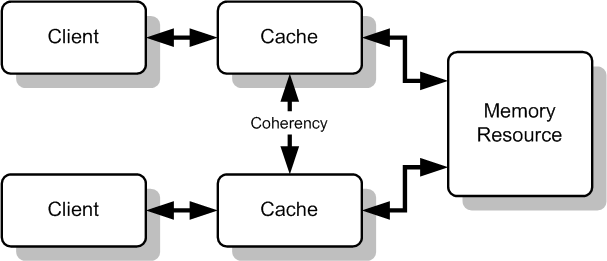
\includegraphics[scale=0.7]{L23/coherency}

    Image courtesy of Wikipedia.
  \end{center}

  \begin{changemargin}{1cm}
  {\bf Coherency:}
  \begin{itemize}
    \item Values in all caches are consistent;
    \item System behaves as if all CPUs are using shared memory.
  \end{itemize}
  \end{changemargin}
\end{frame}
%%%%%%%%%%%%%%%%%%%%%%%%%%%%%%%%%%%%%%%%%%%%%%%%%%%%%%%%%%%%%%%%%%%%%%%%%%%%%%%%

%%%%%%%%%%%%%%%%%%%%%%%%%%%%%%%%%%%%%%%%%%%%%%%%%%%%%%%%%%%%%%%%%%%%%%%%%%%%%%%%
\begin{frame}
  \frametitle{Cache Coherence Example}

  \begin{changemargin}{1cm}
  Initially in main memory: {\tt x = 7}.

  \begin{enumerate}
    \item {\tt CPU1} reads x, puts the value in its cache.
    \item {\tt CPU3} reads x, puts the value in its cache.
    \item {\tt CPU3} modifies {\tt x := 42}
    \item {\tt CPU1} reads x \ldots ~from its cache?
    \item {\tt CPU2} reads x. Which value does it get?
  \end{enumerate}
  ~\\

  Unless we do something, {\tt CPU1} is going to read invalid data.
  \end{changemargin}
\end{frame}
%%%%%%%%%%%%%%%%%%%%%%%%%%%%%%%%%%%%%%%%%%%%%%%%%%%%%%%%%%%%%%%%%%%%%%%%%%%%%%%%

%%%%%%%%%%%%%%%%%%%%%%%%%%%%%%%%%%%%%%%%%%%%%%%%%%%%%%%%%%%%%%%%%%%%%%%%%%%%%%%%
\begin{frame}
  \frametitle{High-Level Explanation of Snoopy Caches}

  \begin{changemargin}{1cm}
  \begin{itemize}
    \item Each CPU is connected to a simple bus.
    \item Each CPU ``snoops'' to observe if a memory location is read or written
      by another CPU.
    \item We need a cache controller for every CPU.
  \end{itemize}
  ~\\
  {\bf What happens?}

  \begin{itemize}
    \item Each CPU reads the bus to see if any memory operation is relevant. If
      it is, the controller takes appropriate action.
  \end{itemize}
  \end{changemargin}
\end{frame}
%%%%%%%%%%%%%%%%%%%%%%%%%%%%%%%%%%%%%%%%%%%%%%%%%%%%%%%%%%%%%%%%%%%%%%%%%%%%%%%%

\section{Write-Through}
%%%%%%%%%%%%%%%%%%%%%%%%%%%%%%%%%%%%%%%%%%%%%%%%%%%%%%%%%%%%%%%%%%%%%%%%%%%%%%%%
\begin{frame}
  \frametitle{Write-Through Cache}

  \begin{changemargin}{1cm}
Simplest type of cache coherence:
  \begin{itemize}
    \item All cache writes are done to main memory.
    \item All cache writes also appear on the bus.
    \item If another CPU snoops and sees it has the same location in
      its cache, it will either {\it invalidate} or {\it update} the
      data.\\ \qquad (We'll be looking at invalidating.)
  \end{itemize}
~\\

    For write-through caches: normally, when you write to an invalidated
    location, you bypass the cache and go directly to memory (aka {\bf
      write no-allocate}).

  \end{changemargin}
\end{frame}
%%%%%%%%%%%%%%%%%%%%%%%%%%%%%%%%%%%%%%%%%%%%%%%%%%%%%%%%%%%%%%%%%%%%%%%%%%%%%%%%

%%%%%%%%%%%%%%%%%%%%%%%%%%%%%%%%%%%%%%%%%%%%%%%%%%%%%%%%%%%%%%%%%%%%%%%%%%%%%%%%
\begin{frame}
  \frametitle{Write-Through Protocol}

  \begin{changemargin}{1cm}
  \begin{itemize}
    \item Two states, {\bf valid} and {\bf invalid}, for each memory location.
    \item Events are either from a processor ({\bf Pr}) or the {\bf Bus}.
  \end{itemize}
  \vfill
  \begin{center}
    \begin{tabular}{llll}
      {\bf State} & {\bf Observed} & {\bf Generated} & {\bf Next State}\\
      Valid   & PrRd  &       & Valid\\
      Valid   & PrWr  & BusWr & Valid\\
      Valid   & BusWr &       & Invalid\\
      Invalid & PrWr  & BusWr & Invalid\\
      Invalid & PrRd  & BusRd & Valid\\
    \end{tabular}
  \end{center}
  \end{changemargin}
\end{frame}
%%%%%%%%%%%%%%%%%%%%%%%%%%%%%%%%%%%%%%%%%%%%%%%%%%%%%%%%%%%%%%%%%%%%%%%%%%%%%%%%

%%%%%%%%%%%%%%%%%%%%%%%%%%%%%%%%%%%%%%%%%%%%%%%%%%%%%%%%%%%%%%%%%%%%%%%%%%%%%%%%
\begin{frame}
  \frametitle{Write-Through Protocol Example}

  \begin{changemargin}{1cm}

  \begin{itemize}
    \item For simplicity (this isn't an architecture course), assume all cache
      reads/writes are atomic.
  \end{itemize}
  \vfill
  {\bf Using the same example as before:}

  Initially in main memory: {\tt x = 7}.

  \begin{enumerate}
    \item {\tt CPU1} reads x, puts the value in its cache. \structure{(valid)}
    \item {\tt CPU3} reads x, puts the value in its cache. \structure{(valid)}
    \item {\tt CPU3} modifies {\tt x := 42}. \structure{(write to memory)}
      \begin{itemize}
        \item \structure{{\tt CPU1} snoops and marks data as invalid.}
      \end{itemize}
    \item {\tt CPU1} reads x, \structure{from main memory. (valid)}
    \item {\tt CPU2} reads x, \structure{from main memory. (valid)}
  \end{enumerate}
  \end{changemargin}
\end{frame}
%%%%%%%%%%%%%%%%%%%%%%%%%%%%%%%%%%%%%%%%%%%%%%%%%%%%%%%%%%%%%%%%%%%%%%%%%%%%%%%%

\section{Write-Back}
%%%%%%%%%%%%%%%%%%%%%%%%%%%%%%%%%%%%%%%%%%%%%%%%%%%%%%%%%%%%%%%%%%%%%%%%%%%%%%%%
\begin{frame}
  \frametitle{Write-Back Cache}

  \begin{changemargin}{.75cm}

  \begin{itemize}
    \item What if, in our example, {\tt CPU3} writes to {\tt x} 3 times?\\[1em]
    \item Main goal: delay the write to memory as long as possible.\\[1em]
    \item At minimum, we have to add a ``dirty'' bit:\\
     \quad Indicates the our data has not yet been written to memory.
  \end{itemize}
  \end{changemargin}

\end{frame}
%%%%%%%%%%%%%%%%%%%%%%%%%%%%%%%%%%%%%%%%%%%%%%%%%%%%%%%%%%%%%%%%%%%%%%%%%%%%%%%%

%%%%%%%%%%%%%%%%%%%%%%%%%%%%%%%%%%%%%%%%%%%%%%%%%%%%%%%%%%%%%%%%%%%%%%%%%%%%%%%%
\begin{frame}
  \frametitle{Write-Back Implementation}

  \begin{changemargin}{1cm}
     The simplest type of write-back protocol (MSI), with 3 states:
      \begin{itemize}
        \item {\bf Modified}---only this cache has a valid copy; \\
          \quad main memory is {\bf out-of-date}.
        \item {\bf Shared}---location is unmodified, \\
          \quad up-to-date with main
          memory; \\
          \quad may be present in other caches (also up-to-date).
        \item {\bf Invalid}---same as before.
      \end{itemize}~\\
      
     Initial state, upon first read, is ``shared''.\\[1em]

     Implementation will only write the data to memory if another
        processor requests it.\\[1em]

     During write-back, a processor may read the data from the bus.
  \end{changemargin}
\end{frame}
%%%%%%%%%%%%%%%%%%%%%%%%%%%%%%%%%%%%%%%%%%%%%%%%%%%%%%%%%%%%%%%%%%%%%%%%%%%%%%%%

%%%%%%%%%%%%%%%%%%%%%%%%%%%%%%%%%%%%%%%%%%%%%%%%%%%%%%%%%%%%%%%%%%%%%%%%%%%%%%%%
\begin{frame}
  \frametitle{MSI Protocol}

  \begin{changemargin}{1cm}
  \begin{itemize}
    \item Bus write-back (or flush) is {\bf BusWB}.
    \item Exclusive read on the bus is {\bf BusRdX}.
  \end{itemize}~\\

  \begin{center}
    \begin{tabular}{llll}
      {\bf State} & {\bf Observed} & {\bf Generated} & {\bf Next State}\\
      Modified   & PrRd   &        & Modified\\
      Modified   & PrWr   &        & Modified\\
      Modified   & BusRd  & BusWB  & Shared\\
      Modified   & BusRdX & BusWB  & Invalid\\
      Shared     & PrRd   &        & Shared\\
      Shared     & BusRd  &        & Shared\\
      Shared     & BusRdX &        & Invalid\\
      Shared     & PrWr   & BusRdX & Modified\\
      Invalid    & PrRd   & BusRd  & Shared\\
      Invalid    & PrWr   & BusRdX & Modified\\
    \end{tabular}
  \end{center}
  \end{changemargin}
\end{frame}
%%%%%%%%%%%%%%%%%%%%%%%%%%%%%%%%%%%%%%%%%%%%%%%%%%%%%%%%%%%%%%%%%%%%%%%%%%%%%%%%

%%%%%%%%%%%%%%%%%%%%%%%%%%%%%%%%%%%%%%%%%%%%%%%%%%%%%%%%%%%%%%%%%%%%%%%%%%%%%%%%
\begin{frame}
  \frametitle{MSI Example}

  \begin{changemargin}{1cm}

  {\bf Using the same example as before:}

  Initially in main memory: {\tt x = 7}.

  \begin{enumerate}
    \item {\tt CPU1} reads x from memory. \structure{(BusRd, shared)}
    \item {\tt CPU3} reads x from memory. \structure{(BusRd, shared)}
    \item {\tt CPU3} modifies {\tt x = 42}:
      \begin{itemize}
        \item \structure{Generates a BusRdX.}
        \item \structure{{\tt CPU1} snoops and invalidates x.}
        \item \structure{{\tt CPU3} changes {\tt x}'s state to modified.}
      \end{itemize}
    \item {\tt CPU1} reads x:
      \begin{itemize}
        \item \structure{Generates a BusRd.}
        \item \structure{{\tt CPU3} writes back the data and sets x to shared.}
        \item \structure{{\tt CPU1} reads the new value from the bus as shared.}
      \end{itemize}
    \item {\tt CPU2} reads x from memory. \structure{(BusRd, shared)}
  \end{enumerate}
  \end{changemargin}
\end{frame}
%%%%%%%%%%%%%%%%%%%%%%%%%%%%%%%%%%%%%%%%%%%%%%%%%%%%%%%%%%%%%%%%%%%%%%%%%%%%%%%%

%%%%%%%%%%%%%%%%%%%%%%%%%%%%%%%%%%%%%%%%%%%%%%%%%%%%%%%%%%%%%%%%%%%%%%%%%%%%%%%%
\begin{frame}
  \frametitle{An Extension to MSI: MESI}

  \begin{changemargin}{1cm}
    The most common protocol for cache coherence is MESI.\\[1em]
    Adds another state:
      \begin{itemize}
        \item {\bf Modified}---only this cache has a valid copy; \\
\qquad main memory is {\bf out-of-date}.
        \item {\bf Exclusive}---only this cache has a valid copy; \\
\qquad main memory is {\bf up-to-date}.
        \item {\bf Shared}---same as before.
        \item {\bf Invalid}---same as before.
      \end{itemize}
~\\

    MESI allows a processor to modify data exclusive to it, \\without
      having to communicate with the bus.\\
    MESI is \structure{safe}: in E state, no other processor has the
      data.
  \end{changemargin}
\end{frame}
%%%%%%%%%%%%%%%%%%%%%%%%%%%%%%%%%%%%%%%%%%%%%%%%%%%%%%%%%%%%%%%%%%%%%%%%%%%%%%%%

%%%%%%%%%%%%%%%%%%%%%%%%%%%%%%%%%%%%%%%%%%%%%%%%%%%%%%%%%%%%%%%%%%%%%%%%%%%%%%%%
\begin{frame}
  \frametitle{Even More States!}

  \begin{changemargin}{1cm}
    MESIF (used in latest i7 processors):
      \begin{itemize}
        \item {\bf Forward}---basically a shared state; but, current
          cache is the only one that will respond to a request to
          transfer the data.
      \end{itemize}~\\[1em]

    Hence: a processor requesting data that is already shared or exclusive will
      only get one response transferring the data.\\[1em]
    Permits more efficient usage of the bus.
  \end{changemargin}
\end{frame}
%%%%%%%%%%%%%%%%%%%%%%%%%%%%%%%%%%%%%%%%%%%%%%%%%%%%%%%%%%%%%%%%%%%%%%%%%%%%%%%%

%%%%%%%%%%%%%%%%%%%%%%%%%%%%%%%%%%%%%%%%%%%%%%%%%%%%%%%%%%%%%%%%%%%%%%%%%%%%%%%%
\begin{frame}
  \frametitle{Good Questions (1)}

  \begin{changemargin}{1cm}
  {\bf Cache coherency seems to make sure my data is consistent. Why do I have
    to have something like flush or fence?}
  \begin{itemize}
    \item You might be ok, if all of the writes on processors are to the
      cache. But they're not!
    \item Cache coherency won't update any values modified in registers.
  \end{itemize}
  \end{changemargin}
\end{frame}
%%%%%%%%%%%%%%%%%%%%%%%%%%%%%%%%%%%%%%%%%%%%%%%%%%%%%%%%%%%%%%%%%%%%%%%%%%%%%%%%

%%%%%%%%%%%%%%%%%%%%%%%%%%%%%%%%%%%%%%%%%%%%%%%%%%%%%%%%%%%%%%%%%%%%%%%%%%%%%%%%
\begin{frame}[fragile]
  \frametitle{Good Questions (2)}

  \begin{changemargin}{1cm}
  {\bf Well, I read that {\tt volatile} variables aren't stored in registers,
    so then am I okay?}
  \vspace{6.2em}
  \pause

  \begin{center}
    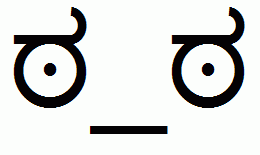
\includegraphics[scale=0.3]{L23/disapproval}    
  \end{center}
  \end{changemargin}
\end{frame}
%%%%%%%%%%%%%%%%%%%%%%%%%%%%%%%%%%%%%%%%%%%%%%%%%%%%%%%%%%%%%%%%%%%%%%%%%%%%%%%%

%%%%%%%%%%%%%%%%%%%%%%%%%%%%%%%%%%%%%%%%%%%%%%%%%%%%%%%%%%%%%%%%%%%%%%%%%%%%%%%%
\begin{frame}[fragile]
  \frametitle{Good Questions (2)}

  \begin{changemargin}{1cm}
  {\bf Well, I read that {\tt volatile} variables aren't stored in registers,
    so then am I okay?}\\[1em]

    {\tt volatile} in C was only designed to:
      \begin{itemize}
        \item Allow access to memory mapped devices.
        \item Allow uses of variables between {\tt setjmp} and {\tt longjmp}.
        \item Allow uses of {\tt sig\_atomic\_t} variables in signal handlers.
      \end{itemize}~\\[1em]
    Remember, things can also be reordered by the compiler,
      {\tt volatile} doesn't prevent this.\\[1em]
    Also, it's likely your variables could be in registers the majority
      of the time, except in critical areas.
  \end{changemargin}
\end{frame}
%%%%%%%%%%%%%%%%%%%%%%%%%%%%%%%%%%%%%%%%%%%%%%%%%%%%%%%%%%%%%%%%%%%%%%%%%%%%%%%%

%%%%%%%%%%%%%%%%%%%%%%%%%%%%%%%%%%%%%%%%%%%%%%%%%%%%%%%%%%%%%%%%%%%%%%%%%%%%%%%%
\begin{frame}
  \frametitle{Cache Coherency Summary}

  \begin{changemargin}{1cm}
    We saw the basics of cache coherence (good to know, but more of an architecture
      thing).\\[1em]
    There are many other protocols for cache coherence, each with their own
      trade-offs.\\[1em]

     Recall: OpenMP flush acts as a {\bf memory barrier/fence} so the
      compiler and hardware don't reorder reads and writes.\\[1em]
    \begin{itemize}
     \item Neither cache coherence nor {\tt volatile} will save you.
    \end{itemize}

  \end{changemargin}
\end{frame}
%%%%%%%%%%%%%%%%%%%%%%%%%%%%%%%%%%%%%%%%%%%%%%%%%%%%%%%%%%%%%%%%%%%%%%%%%%%%%%%%

\end{document}
